\section{Konfiguration}

Die Konfigurationsseite erlaubt es neben der ACP-Nutzerkontoverwaltung ebenfalls ganz grundlegende Einstellungswerte für das Sokka-System festzulegen.

\begin{figure}[ht]
    \centering
    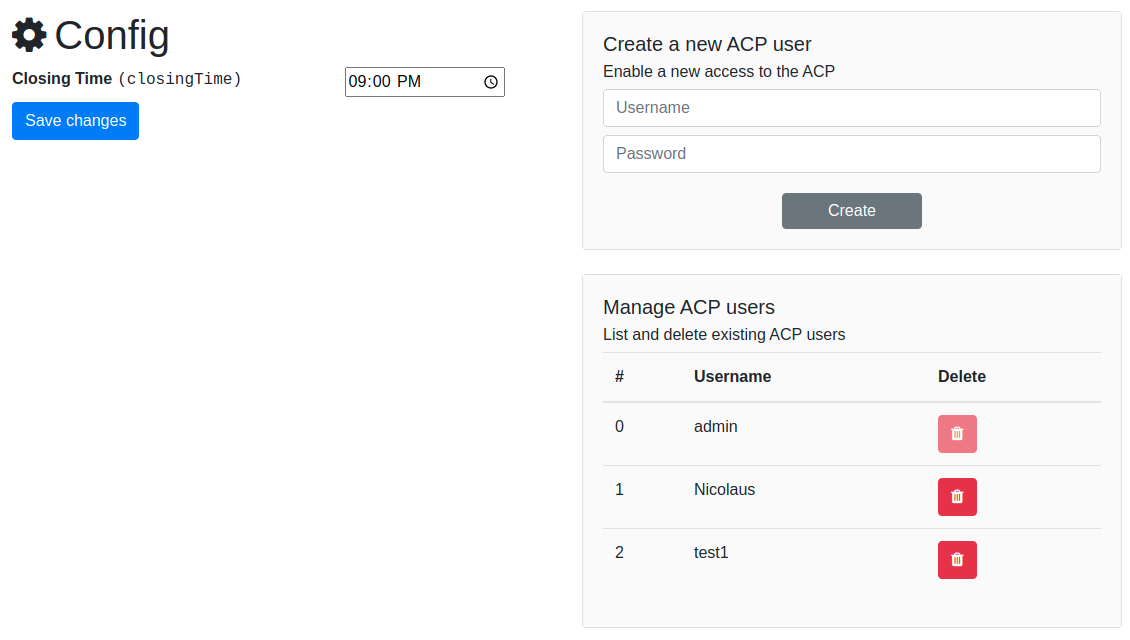
\includegraphics[width=0.8\textwidth]{images/ACP/config.png}
    \caption{Die Konfigurationsseite des Sokka-ACPs}
\end{figure}

Die Funktionsweise der Nutzerverwaltung wird in der Sektion \textit{\nameref{acp-usersystem}} genauer erläutert.

Zum Zeitpunkt des Schreibens gibt es auf dieser Seite nur eine Einstellung. Diese ist die \lstinline{closingTime}, welche jene Uhrzeit ist, zu der keine Bestellungen für den folgenden Tag zulässig sind. Ist die \lstinline{closingTime} beispielsweise \textit{9:00 PM}, so ist es Nutzern maximal bis 21:00 Uhr möglich Bestellungen zu tätigen, andernfalls erhalten sie im Client eine Fehlermeldung.

\begin{figure}[ht]
    \centering
    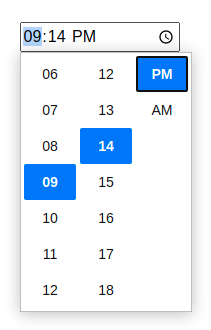
\includegraphics[width=0.2\textwidth]{images/ACP/config_date.png}
    \caption{Die Zeitauswahl auf der Konfigurationsseite im Sokka-ACP}
\end{figure}

Das Format der Zeit im Input-Feld passt sich dem Format des Computers an, von dem auf das ACP zugegriffen wird.